\chapter{Termodinamica}

Passiamo ora a studiare la termodinamica, che è la branca della fisica che studia le trasformazioni di energia e il calore. Quando trattiamo di termodinamica solitamente ci riferiamo a sistemi macroscopici, cioè sistemi composti da un numero molto elevato di particelle, questo numero è ben descritto dalla costante di Avogadro ($N_A=6\cdot 10^{23}$) questo è un numero puro. Il numero di Avogadro è il numero di atomi o molecole contenuti in un grammo di sostanza dunque se abbiamo $N$ particelle in un sistema allora $N\rightarrow n=\frac{N}{N_A}$ è il numero di moli ($\operatorname{mol}$). Le moli sono una grandezza fondamentale per indicare la quantità di sostanza. Altre grandezze fondamentali quando trattiamo di termodinamica sono la densità di massa $\rho = \frac{m}{V}$ misurata in $\left[\frac{M}{L^3}\right]=\frac{kg}{m^3}$, la densità molare $m \stackrel{def}= \frac{n}{V}$ misurata in $\left[\frac{M}{L^3}\right]=\frac{mol}{m^3}$, la pressione che è una quantità scalare che indica la forza esercitata su una superficie, è definita come il rapporto tra la forza e l'area su cui essa agisce, $P\stackrel{def}{=}\frac{\left| \vec{F_{\perp,s}}\right|}{S}$, misurata in $\left[\frac{M}{L^2T^2}\right]=\frac{N}{m^2}=\frac{kg}{m\cdot s^2}$. La pressione oltre ad avere dimensionalità di $\left[\frac{F}{L^2}\right]$ può essere espressa come \textit{Pascal} ($\frac{1\ \operatorname{N}}{1\ \operatorname{m}^2}=1\operatorname{Pa}$ dato che tale quantità è insignificante sono state istituite le misure di $1\operatorname{bar}=10^5\operatorname{Pa}$ e $1\operatorname{atm}=1013.25\operatorname{bar}$). Infine l'ultima grandezza fisica che necessita un'introduzione prima di passare al capitolo è la temperatura, questa può essere espressa in Kelvin ($K$) o Celsius ($^{\circ}C$) e la conversione tra le due scale è data da $T(K)=t(^{\circ}C)+273.15$. 
\subsubsection{Calcolo della pressione}
    Assumiamo di voler calcolare la pressione esercitata da un'insieme di particelle su una parete che le contiene. Per prima cosa dobbiamo assumere che: \begin{enumerate}
        \item $m_i \leftrightarrow m_j$ non interagiscono tra di loro per ogni $i,j \in [1,N]$.
        \item Gli urti tra particella e parete sono perfettamente elastici, inoltre la massa della parete è molto maggiore di quella delle particelle ($M\gg m$)
        \item Il raggio della particella è trascurabile
    \end{enumerate}
    Avendo assunto tutto ciò chiameremo $``P_{\text{lungo} x}''$ la pressione esercitata dalle particelle lungo l'asse $x$, la pressione che una singola particella esercita sulla parete è data da: $P_{\text{lungo } x}=\frac{F_{\text{lungo} x}}{L_y\cdot L_z}$, dove $F_{\text{lungo} x}$ è la forza esercitata dalla particella sulla parete e $L_y\cdot L_z$ è l'area della parete. La forza esercitata dalla particella sulla parete è una forza impulsiva dunque si dovrebbe calcolare come $-\frac{J}{\Delta t}$ dato che l'intervallo di tempo da considerare nella situazione di impulso è molto piccolo, consideriamo equivalentemente $\Delta t$ come il periodo tra due urti sulla stessa parete, questa sarà $\Delta t=\frac{2L_x}{v_x}$ che è il tempo per percorrere due volte la lunghezza $L_x$ con componente della velocità $v_x$. Passano al denominatore l'impulso $J$ è dato da $J=(P_{f,x}-P_{i,x})\cdot \hat{x}$ ma dato che $P_{f,x}=-P_{i_x}$ visto che gli urti sono completamente elastici ed la massa della superficie è molto maggiore rispetto alla massa della particella, dunque $``F_{\text{lungo } x}''=\frac{m v_x^2}{L_x}$ il che significa che la pressione lungo la superficie $L_y\cdot L_z$ è $P_{\text{lungo }x} = \frac{\frac{m v_x^2}{L_x}}{L_y\cdot L_z} = \frac{m_iv_x^2}{L_xL_yL_z}=\frac{m_iv_x^2}{V}$. Questo vale solo per una particella, sommando l'insieme delle particelle otteniamo:
    \begin{align*}
        \sum_{i=1}^N\frac{m_iv_{x,i}^2}{V}=&\frac{m}{V}N\frac{\sum_{i=1}^N v_{x,i}}{N}
        =&\frac{Nm<v_x^2>}{V}
    \end{align*}
    Notiamo come $N,m,V$ siano uguali per tutti gli assi e l'unico parametro che cambi sia la velocità di tutte le particelle sull'asse $x$ tuttavia dato che il sistema complessivamente è isotropo possiamo dire che $<v_x^2>=<v_y^2>=<v_z^2>$ e quindi possiamo scrivere la pressione totale come:
    \begin{align}
        P = \frac23\frac{N<E_x>}{V}
    \end{align}
    dove $<E_x>$ è l'energia cinetica media lungo l'asse $x$ e $N$ è il numero di particelle. 
\section{Calore}
    Abbiamo accennato alla temperatura, possiamo dire che che la differenza di temperatura sia proporzionale alla massa del materiale combustibile usato, ($\Delta T \propto m_{comb}$), infatti logicamente più combustibile abbiamo più calore possiamo generare per una stessa quantità da scaldare. Inoltre se la massa del corpo da scaldare è proporzionale alla massa del combustibile, ($M_{scaldato} \propto m_{comb}$) infatti con più massa da scaldare abbiamo bisogno di più calore per scaldarlo della stessa temperatura. Infine possiamo dire che il calore $\mathcal{Q}$ è proporzionale alla differenza di temperatura ($\Delta T$) e alla massa del corpo da scaldare ($M_{scaldato}$), quindi possiamo scrivere:
    $$
        \mathcal{Q}=cm\Delta T
    $$
    Dove $c$ è il calore specifico, che è una costante che dipende dal materiale e dalla temperatura. Il calore specifico è definito come la quantità di calore necessaria per aumentare la temperatura di un'unità di massa di un materiale di un grado Celsius. La sua unità di misura è $\frac{J}{kg\cdot K}$. Il calore ha la stessa dimensionalità dell'energia, infatti viene misurato in Joule ($J$). 
    \subsubsection{Esperimento di Joule}
        Prendiamo in considerazione un contenitore isolato termicamente, nel quale è presente un pistone ed un liquido in esso. Il pistone è collegato tramite delle carrucole ideali ad un peso $P$ che scende di un'altezza $h$. Dunque il lavoro compiuto dal peso è $W=-P\cdot (h_f -h_i)$ in quanto $E_{pot,i}=-P\cdot h_i$ e $E_{pot,f}=-P\cdot h_f$ e quindi dato che $h_f<h_i$ allora $mgh_i>mgh_f$ dunque $\Delta U_m = mg(h_f-h_i<0$. È quindi compiuto un lavoro dal peso sul liquido il quale ne aumenta l'energia potenziale dunque $\Delta U_{H_2O} > 0$  per questo possiamo dire che:
        \begin{align}
            W &= \Delta U \propto \Delta T_{H_2O}\\
            \mathcal{Q} &= m_{H_2O}c_{H_2O}\Delta T_{H_2O}\\
            \Delta U_{H_2O} &= \mathcal{Q} - W \label{eq:prima_legge_termo}
        \end{align}
        L'equazione \ref{eq:prima_legge_termo} è nota come prima legge della termodinamica, essa afferma che l'energia interna di un sistema è uguale alla somma del calore fornito al sistema e del lavoro compiuto sul sistema. Essa è una legge fondamentale della termodinamica e rappresenta il principio di conservazione dell'energia applicato ai sistemi termodinamici.\newline
        Per convenzione si considera il calore fornito al sistema come positivo e il lavoro compiuto sul sistema come positivo, di conseguenza il calore ceduto dal sistema e il lavoro compiuto dal sistema sono considerati negativi. La prima legge della termodinamica può essere espressa in forma differenziale come:
        \begin{align*}
            dU = \delta Q - \delta W
        \end{align*}
        non possiamo usare il simbolo $d$ per il calore e il lavoro perché non sono funzioni di stato, ma dipendono dal ``percorso'' seguito dal sistema per passare da uno stato all'altro.\newline
        Se quindi viene eseguito un lavoro sul sistema e il calore viene fornito al sistema, l'energia interna del sistema aumenta. Se invece il sistema compie lavoro e cede calore, l'energia interna del sistema diminuisce. La prima legge della termodinamica è una legge fondamentale della fisica e ha molte applicazioni in ingegneria, chimica e fisica. Essa è alla base della termodinamica e delle sue applicazioni pratiche, come i motori a combustione interna, le turbine a gas e le pompe di calore.
\section{Stato Termodinamico}
    Un sistema termodinamico è definito da un insieme di variabili macroscopiche che descrivono il suo stato. Queste variabili sono chiamate variabili di stato e includono grandezze come la temperatura, la pressione, il volume e la massa del sistema, ma anche altre. Lo stato del sistema viene espresso come $f(v_1,v_2,\dots,v_n)=0$ dove $v_i$ sono le variabili del sistema termodinamico. L'uguaglianza a zero sta ad indicare che il sistema è in equilibrio termodinamico, se non fosse così il sistema non sarebbe in equilibrio e quindi il suo stato non sarebbe definito, infatti nelle trasformazioni termodinamiche si passa da uno stato $s_1$ ad uno stato $s_2$ ($s_1\rightarrow s_2$) e quindi il sistema non è più in equilibrio.
    \paragraph{Equilibrio Termodinamico}
        Un sistema è in equilibrio termodinamico se sono vere tre condizioni:
        \begin{enumerate}
            \item Sussiste un equilibrio meccanico \underline{medio} tra le particelle del sistema. 
            \item Sussiste un equilibrio chimico tra le particelle del sistema.
            \item Sussiste un equilibrio termico \underline{medio} tra le particelle del sistema.
        \end{enumerate}
        I punti 1 e 3 sono stati definiti \textit{equilibrio medio} poiché non è necessario che ogni singola particella del sistema sia in equilibrio, ma è sufficiente che nel complesso il sistema sia ``fermo'' o a ``temperatura costante''. In particolare, l'equilibrio termico medio implica che la temperatura del sistema sia uniforme e costante nel tempo. Se il sistema non è in equilibrio, le variabili di stato possono variare nel tempo e il sistema può subire trasformazioni termodinamiche. In questo caso, le variabili di stato non sono più costanti e il sistema non è più in equilibrio, l'equazione di stato non sarà più valida.
    \subsection{Trasformazioni termodinamiche}
        Andiamo ora a definire le trasformazioni termodinamiche, esse sono i processi attraverso i quali un sistema termodinamico passa da uno stato iniziale a uno stato finale. Le trasformazioni termodinamiche possono essere classificate in base a diverse caratteristiche, come la natura del processo (reversibile o irreversibile), la variazione di temperatura (isoterma, adiabatica, isocora, isobara) e la variazione di energia interna (isocora, isobara). 
        \subsubsection{Trasformazioni Adiabatiche}
            Le trasformazioni adiabatiche sono processi in cui non c'è scambio di calore tra il sistema e l'ambiente circostante. Ovvero $\mathcal{Q}=0$ e quindi $\Delta U = -W$. In questo caso, l'energia interna del sistema può variare solo a causa del lavoro compiuto sul sistema o dal sistema. Le trasformazioni adiabatiche sono caratterizzate da una variazione di temperatura e pressione, ma non da una variazione di calore. Un esempio di trasformazione adiabatiche è l'espansione rapida di un gas in un cilindro, in cui il gas si espande senza scambiare calore con l'ambiente circostante.
        \subsubsection{Trasformazioni non-diabatiche}
            Le trasformazioni dove c'è scambio di calore tra il sistema e l'ambiente circostante sono dette non-adiabatiche. Un oggetto o un sistema può essere scaldato o raffreddato in diversi modi
                \paragraph{Conduzione di calore} 
                    La conduzione di calore è il processo attraverso il quale il calore viene trasferito da un corpo a un altro attraverso il contatto diretto. In questo caso il calore è proporzionale alla superficie di contatto: $S\propto Q$, al tempo per il quale il calore viene trasferito: $\delta t\propto Q$, alla differenza di temperatura tra i due corpi: $\Delta \mathcal{T}\propto Q$ ed infine ad un coefficiente di conduzione del materiale: $k\propto Q$ il quale oltre a dipendere dal materiale dipende anche dalla temperatura. Dunque possiamo scrivere:
                    \begin{align}
                        \mathcal{Q}=h(T_2-T_1)S\Delta t
                    \end{align}
                    portando l'equazione in forma differenziale otteniamo:
                    \begin{align}
                        dQ = -\frac{d\mathcal{T}}{dm}ds\, dt\, k \label{eq:legge_furier}
                    \end{align}
                    dove $dQ$ è il calore trasferito, $dm$ è la massa del materiale, $ds$ è lo spessore del materiale e $dt$ è il tempo di conduzione. L'equazione \ref{eq:legge_furier} è nota come legge di Fourier per la conduzione del calore. Essa descrive il flusso di calore attraverso un materiale in funzione della differenza di temperatura, dello spessore del materiale e del tempo di conduzione. La legge di Fourier è alla base della termodinamica e ha molte applicazioni pratiche, come l'isolamento termico degli edifici e la progettazione di scambiatori di calore.
                \paragraph{Convezione}
                    La convezione è il processo attraverso il quale il calore viene trasferito da un corpo a un altro attraverso il movimento di un fluido. Non andremo ad analizzare nel dettaglio questo processo poiché questo è molto complesso e non rientra nello scopo del corso.
                \paragraph{Irraggiamento}
                    L'irraggiamento è il processo attraverso il quale il calore viene trasferito da un corpo a un altro attraverso l'emissione di radiazioni elettromagnetiche. Questo processo avviene senza contatto diretto tra i corpi e senza la necessità di un fluido intermedio. L'irraggiamento è responsabile del trasferimento di calore dal Sole alla Terra e da un corpo caldo a uno freddo. La legge di Stefan-Boltzmann descrive come il calore trasferito $\epsilon$ da un corpo a un altro attraverso l'irraggiamento è proporzionale alla quarta potenza della temperatura assoluta del corpo emittente, e all'efficienza del corpo ricevente $\ell$:
                    \begin{align*}
                        \epsilon = \ell \cdot \sigma \cdot (T^4)
                    \end{align*}
                    dove $\sigma$ è la costante di Stefan-Boltzmann, che ha un valore di circa $5.67 \cdot 10^{-8} \frac{W}{m^2 \cdot K^4}$. La legge di Stefan-Boltzmann è alla base della termodinamica e ha molte applicazioni pratiche, come la progettazione di pannelli solari e il riscaldamento degli edifici
        \subsubsection{Cambi di fase}
            Un caso particolare nel quale una variazione di calore non comporti una variazione di temperatura è il passaggio di stato, ovvero il passaggio da uno stato fisico a un altro. Ad esempio, quando si riscalda dell'acqua, essa passa dallo stato solido (ghiaccio) a quello liquido (acqua) e poi a quello gassoso (vapore). Durante questo processo, la temperatura dell'acqua rimane costante fino a quando tutto il ghiaccio non si è sciolto e poi rimane costante fino a quando tutto l'acqua non è evaporata. Questo fenomeno è dovuto al fatto che il calore fornito al sistema viene utilizzato per rompere i legami tra le molecole del ghiaccio o dell'acqua, piuttosto che per aumentare la temperatura del sistema. Il calore necessario per il passaggio di stato è chiamato calore latente e dipende dalla sostanza, dalla temperatura e dalla pressione. Il calore latente di fusione è il calore necessario per passare dallo stato solido a quello liquido, mentre il calore latente di vaporizzazione è il calore necessario per passare dallo stato liquido a quello gassoso.
            \paragraph{Il grafico dello stato della materia}
                Lo stato di un materiale può essere riassunto in un grafico nel quale sull'asse ``$x$'' la temperatura e sull'asse ``$y$'' la pressione. In questo grafico è presente un punto denominato punto triplo ($T_{tr}$) che è il punto in cui coesistono i tre stati della materia (solido, liquido e gassoso). 
                \begin{figure}[H]
                    \centering
                    \begin{tikzpicture}[scale=1.2, font=\small]
                        \draw[->] (0,0) -- (10,0) node[right] {$T (\operatorname{K})$};
                        \draw[->] (0,0) -- (0,7) node[above] {$P (\operatorname{atm})$};
                        
                        % Etichette sugli assi (temperature)
                        \foreach \x/\xlabel in {1/250, 2/273, 4/373, 9/647}
                        \draw (\x,0.1) -- (\x,-0.1) node[below] {\xlabel};
                        
                        % Etichette pressione (approssimazione visiva)
                        \foreach \y/\ylabel in {1/0.006, 2/1, 4/100, 6/200, 7/218}
                        \draw (0.1,\y) -- (-0.1,\y) node[left] {\ylabel};
                        
                        % Punto triplo (273.16 K, 0.006 atm)
                        \filldraw[red] (2,1) circle (2pt) node[above right] {Punto triplo};
                        
                        % Punto critico (647 K, 218 atm)
                        \filldraw[blue] (9,7) circle (2pt) node[above left] {Punto critico};
                        
                        % Linea solido-liquido
                        \draw[thick] (1,6) -- (2,1);
                        
                        % Linea liquido-gas
                        \draw[thick] (2,1) .. controls (4,2) and (6,3.5) .. (9,7);
                        
                        % Linea solido-gas
                        \draw[thick] (2,1) .. controls (1,0.5) and (0.5,0.2) .. (0.2,0.05);
                        
                        % Etichette delle fasi
                        \node at (0.8,4.5) {Solido};
                        \node at (4,3.2) {Liquido};
                        \node at (5,0.5) {Vapore};
                        
                    \end{tikzpicture}
                \end{figure}
                Il grafico mostra le diverse fasi della materia in funzione della temperatura e della pressione. La linea che separa il solido dal liquido è chiamata linea di fusione, mentre la linea che separa il liquido dal vapore è chiamata linea di vaporizzazione. La linea che separa il solido dal vapore è chiamata linea di sublimazione. Il punto critico è il punto oltre il quale non è possibile distinguere tra liquido e vapore, e oltre il quale il materiale si comporta come un fluido supercritico. Inoltre al disotto di una certa pressione e temperatura non si può avere dell'acqua intesa come $H_2O$ ma la materia si decompone in idrogeno e ossigeno.
            \paragraph{Cambio di fase analiticamente}
                Analiticamente il cambio di fase può essere descritto come:
                \begin{align}
                    -\lambda m = \mathcal{Q}
                \end{align}
                Dove come già accennato $\lambda$ è il calore latente di fusione o vaporizzazione e $m$ è la massa del materiale da scalare/raffreddare. 
    \subsection{Altre leggi che regolano la termodinamica}
        Rimanendo nel campo dello stato termodinamico nel corso degli anni sono state formulate delle leggi che ne regolano il comportamento. Oltre alla prima legge della termodinamica abbiamo la legge di Avogadro, la legge di Boyle e le leggi di Gay-Lussac che regolano il comportamento dei gas ideali.
        \begin{definition}[Legge di Avogadro - Gas Ideali]
            Il numero di moli di un gas ideale è dipendente dalla pressione, dal volume e dalla temperatura del gas stesso.\newline
            Nelle stesse condizioni di temperatura e pressione, volumi uguali di gas diversi contengono lo stesso numero di molecole.
        \end{definition}
        \begin{definition}[Legge di Boyle - Gas Ideali]
            La legge di Boyle afferma che a temperatura costante, il prodotto pressione-volume di un gas ideale è costante. In altre parole, se la temperatura di un gas ideale rimane costante, un aumento della pressione del gas comporta una diminuzione del volume e viceversa.
            \begin{align}
                PV = \text{costante} \label{eq:legge_boyle}
            \end{align}
        \end{definition}
        \begin{definition}[1° Legge di Gay-Lussac - Gas Ideali]
            A pressione costante, il volume di un gas ideale è dipende dalla temperatura.
            \begin{align}
                P = \text{costante} \Rightarrow V(t)=V_0\left[1+\alpha(T-T_0)\right]
            \end{align}
        \end{definition}
        \begin{definition}[2° Legge di  Gay-Lussac - Gas Ideali]
            A volume costante, la pressione di un gas ideale è dipendente dalla temperatura.
            \begin{align}
                V = \text{costante} \Rightarrow P(t)=P_0\left[1+\beta(T-T_0)\right]
            \end{align}
        \end{definition}
        Queste quattro leggi sono alla base della termodinamica e sono utilizzate per descrivere il comportamento dei gas ideali. Unendole quindi possiamo ricavarci l'equazione di stato per i gas ideali:
        \begin{align}
            PV = nRT \label{eq:gas_ideale}
        \end{align}
        dove $P$ è la pressione, $V$ è il volume, $n$ è il numero di particelle (solitamente in moli) e $R$ è la costante universale dei gas ideali, che ha un valore di circa $8.314 \frac{J}{mol \cdot K}$ ed infine $T$ è la temperatura in Kelvin.\newline 
        L'equazione di stato dei gas ideali (\ref{eq:gas_ideale}) scritta in formato molare è:
        \begin{align}
            PV = Mk_{B}T
        \end{align}
        la quale sfrutta la costante \underline{naturale} di Boltzmann ($k_B$) che ha un valore di circa $1.38 \cdot 10^{-23} \frac{J}{K}$ e $M$ è la massa molare del gas in $\frac{kg}{mol}$. A differenza del numero di Avogadro ($N_A$) che è un numero puro \underline{arbitrario} e non ha unità di misura, la costante di Boltzmann è una costante fisica fondamentale che ha un valore specifico e una dimensione fisica.
        \subsubsection{Gas Ideali}
            Un gas ideale è un modello teorico di un gas che segue le leggi prima descritte ed è caratterizzato dal'equazione di stato $PV-nRT = 0$. Per essere ideale un gas ``generalmente'' deve essere rarefatto, ovvero le particelle devono essere distanti tra di loro e non devono interagire tra di loro. Inoltre vanno trascurate le forze intermolecolari e le dimensioni delle particelle. In questo modo possiamo descrivere una teoria cinetica dei gas, che ci permette di calcolare la pressione, il volume e la temperatura del gas in funzione delle sue proprietà microscopiche. 
            \paragraph{Densità dell'aria}
                Dato che come accennato l'aria è un gas ideale possiamo calcolarne la densità usando l'equazione di stato dei gas ideali. Questa sarà data da:
                \begin{align*}
                    \rho &= \frac{m}{V}\\
                    &= \frac{m_{\text{particella}}N}{V}\\
                    &= \frac{m_{\text{particella}}P\cancel{V}}{\cancel{V}k_{B}T}\\
                    &= \frac{m_{\text{particella}}P}{k_{B}T}
                \end{align*}
                Sapendo che la massa di una singola particella di aria è $m_{\text{particella}}=28.8\cdot 10^{-3}kg$ e che la pressione atmosferica è $P=101325Pa$ e che la temperatura media dell'aria è $T=293K$ possiamo calcolare la densità dell'aria:
                \begin{align*}
                    \rho &= \frac{28.8\cdot 10^{-3}kg\cdot 101325Pa}{1.38\cdot 10^{-23}J/K\cdot 293K}\\
                    &= 1.2\frac{kg}{m^3}
                \end{align*}
\section{Lavoro termodinamico e energia interna}
    \subsection{Lavoro dei gas ideali}
        In senso meccanico il lavoro è definito come il prodotto tra la forza e lo spostamento ($dw=\vec{F}\cdot d\vec{s}$) ma come abbiamo visto in precedenza il lavoro nel senso termodinamico viene definito come il prodotto tra la pressione e il volume ($dW=P\cdot dV$) dimostriamo ora che i due lavori sono equivalenti con l'ausilio di un pistone.
        \begin{proof}
            Consideriamo un pistone isolato termicamente, nel quale è presente un gas ideale, sperimentalmente osserviamo che il pistone non si muove e dunque la risultante delle forze a lui applicate è nulla.\newline
            Dunque la forza peso del pistone stesso è contrastata dalla forza che il gas esercita su di esso ($R=m\vec{g}+\vec{F_{gas}}=\vec{0}$). Ora sembrerebbe che sussista una accelerazione del gas sull'asse $z$ in quanto questa dovrebbe contrastare la forza peso del pistone stesso, tuttavia ciò andrebbe contro l'assunzione che sia presente un gas ideale. Infatti con un gas ideale sussiste l'isotropia delle forze e quindi la forza peso del pistone non può essere contrastata da una forza che agisce solo lungo l'asse $z$ ma deve essere contrastata da una forza che agisce lungo tutti gli assi. Sapendo che la velocità media del gas ideale su una superficie è $<v^2>=630 \frac{m^2}{s^2}$ ed inoltre che questa è opposta ad una accelerazione $g$ della gravità, possiamo dire che la velocità finale dopo un istante $t_1$ è:
            \begin{align*}
                v_{f} = v_0 + g t_1
            \end{align*}
            dove $v_0$ è la velocità iniziale del gas ideale. Sappiamo inoltre che la posizione finale del gas ideale è:
            \begin{align*}
                s_{f} = s_0 + v_0 t_1 + \frac{1}{2} g t_1^2
            \end{align*}
            dove $s_0$ è la posizione iniziale del gas ideale. 
            Dunque la forza peso del pistone è contrastata dalla forza che il gas esercita su di esso ($R=m\vec{g}+\vec{F_{gas}}=\vec{0}$) e quindi possiamo scrivere:
            \begin{align*}
                R = m\vec{g} + \vec{F_{gas}} = 0
            \end{align*}
            Ora assumendo che venga aggiunto un peso di massa $m$ al pistone, allora il pistone si muoverà di una distanza $l$ lungo l'asse $z$, viene quindi compiuto un lavoro $W$ sul sistema (dato che il pistone si abbassa) e quindi possiamo scrivere:
            \begin{align*}
                dw &= \vec{F}_{\text{gas}} \cdot d\vec{l} \\
                &= \vec{F}^{\text{gas}}_{\perp} \cdot d\vec{l} \\
                &= p \cdot \vec{S} \cdot d\vec{l} \\
                &= p \cdot dV
            \end{align*}
            è stato possibile eseguire il passaggio da $F_{gas}$ a $p\cdot S$ in quanto la definizione di pressione è data da $P=\frac{F}{S}$ e quindi $F=P\cdot S$. Inoltre il passaggio da $p\cdot S \cdot d\vec{l}$ a $p\cdot V$ è dovuto al fatto che il pistone si muove lungo l'asse $z$ e quindi la variazione di volume del gas ideale è data da $V=S\cdot d\vec{l}$.
        \end{proof}
    \subsection{Lavoro termodinamico}
        Il lavoro termodinamico è il lavoro compiuto da un sistema termodinamico per passare da uno stato iniziale a uno stato finale. Il lavoro termodinamico viene preso, a differenza del lavoro inteso in senso meccanico, come l'integrale della variazione di pressione rispetto alla variazione di volume del sistema. Il lavoro termodinamico è dato da:
        \begin{align}
            W_{a\rightarrow b}=\int_{A}^{B} p(V) dV
        \end{align}
        quindi intrinsecamente stiamo considerando la somma di tutti i piccolissimi lavori compiuti dal sistema per passare da uno stato iniziale a uno stato finale, dunque in teoria potremmo considerare ognuno di questi inter-stati come uno stato di equilibrio. Tuttavia in certe circostanze non è possibile considerare il sistema ``in equilibro'' in certi stati intermedi. Quando, invece, il sistema è in equilibrio in ogni stato intermedio chiameremo la trasformazione \textbf{quasi-statica} dato che ogni micro stato è in equilibrio. Dunque dato che $p=\frac{mRT}{V}$ possiamo definire:
        \begin{align}
            W_{a\rightarrow b}\stackrel{\operatorname{def}}{=}\int_{A}^{B} mRT \cdot \frac{dV}{V}
        \end{align}

    \subsection{Energia interna ai gas}
        Sperimentalmente consideriamo un contenitore isolato termicamente, nel quale è presente un gas ideale in equilibrio in una metà del contenitore e il vuoto nell'altra metà. Se ora andiamo a rompere il setto che divide le due metà, il gas si espanderà nella metà vuota del contenitore. Durante questo processo il volume che il gas occupa raddoppia, osserviamo che la pressione di questo gas dimezza ma la temperatura rimane costante. Notiamo come nessun lavoro è stato compiuto sul gas e nessun calore è stato scambiato con l'ambiente circostante. Ma in quanto sia la pressione che il volume sono cambiati allora possiamo dire che l'energia interna del sistema dipende solo dalla temperatura e non dal volume o dalla pressione. Dunque possiamo scrivere:
        \begin{align*}
            \left.\begin{aligned}
                U_i = U_f\\
                T_i = T_f
            \end{aligned}\right\}\Rightarrow U=U(T)
        \end{align*}
        Dunque possiamo dire che l'energia interna di un gas ideale è una funzione della temperatura e non del volume o della pressione.\newline
        Altra osservazione che possiamo fare sul sistema è quella che l'energia interna del sistema è una funzione di stato, ovvero non dipende dal percorso seguito dal sistema per passare da uno stato iniziale a uno stato finale, ciò a differenza del lavoro e del calore che sono funzioni di percorso. Infatti se consideriamo due stati $A$ e $B$ del sistema, possiamo passare da $A$ a $B$ in diversi modi, ad esempio attraverso una trasformazione isocora o isobara. Tuttavia l'energia interna del sistema sarà sempre la stessa, indipendentemente dal percorso seguito ma non sarà mai la stessa per il lavoro e il calore. Dunque possiamo scrivere:
        \begin{align*}
            d U = \delta \mathcal{Q} - \delta W
        \end{align*}
        al posto di usare la notazione infinitesimale errata per il calore e il lavoro.
        \subsubsection{Relazione di Mayer}
            La relazione di Mayer è una relazione che descrive, in una trasformazione isocora, la variazione di energia interna di un gas ideale in funzione della sua temperatura e del suo volume. Essa viene ricavata a partire dall'equazione di stato dei gas ideali e dalla definizione di energia interna:
            \begin{align*}
                nc_pdT &= nc_VdT + P dV \\
            \end{align*}
            Differenziando l'equazione di stato dei gas ideali
            \begin{align*}
                pdV + Vdp &= nRdT
            \end{align*}
            Dato che in trasformazione isobara $dp=0$ 
            \begin{align}
                nc_pdT &= nc_VdT + nRdT\\
                \Rightarrow c_p - c_V &= R \label{eq:relazione_mayer}
            \end{align}
            ovvero $c_p$, il calore specifico a pressione costante, è maggiore del calore specifico a volume costante $c_V$ di una quantità pari alla costante universale dei gas ideali $R$. 
\section{Trasformazioni gas ideali}
    Come dalla relazione di Mayer, possiamo considerare ``gas ideali'' quei gas che hanno $c_p>c_V$ e che questi siano indipendenti dalla temperatura.
    \subsection{Trasformazioni adiabatiche}
        Il contenitore isolato termicamente è un sistema chiuso, in cui non c'è scambio di calore con l'ambiente circostante. In questo caso solo il lavoro può essere compiuto nel sistema (tramite una parete mobile) e quindi, tra due punti di equilibro $A$ e $B$, possiamo scrivere:
        \begin{align}
            W_{AB}=-\Delta U = -nc_V(T_B-T_A)=\frac{1}{\gamma-1}(p_aV_a-p_bV_b)
        \end{align}
        dove $\gamma=\frac{c_p}{c_V}$ è il rapporto tra il calore specifico a pressione costante e il calore specifico a volume costante.
        \paragraph{Trasformazione reversibile}
            Se la trasformazione è reversibile, possiamo scrivere:
            \begin{align*}
                d\mathcal{Q} = dU + dW = nc_VdT + pdV = 0
            \end{align*}
            in quanto la trasformazione è reversibile, possiamo usare l'equazione di stato per ognuno degli stati intermedi e dunque la pressione è esprimibile come $p=\frac{nRT}{V}$ e quindi:
            \begin{align*}
                nc_VdT + \frac{nRT}{V}dV = 0
            \end{align*}
            usando l'equazione \ref{eq:relazione_mayer} possiamo scrivere:
            \begin{align*}
                \frac{c_p - c_V}{c_V}\frac{dv}{V} + \frac{dT}{T} = 0 \Rightarrow (\omega-1)\frac{dv}{V} + \frac{dT}{T} = 0
            \end{align*}
            È quindi questa l'equazione che regola ogni coordinata delle trasformazioni adiabatiche reversibili. Integrando da $A$ a $B$ otteniamo:
            \begin{align*}
                \int_{T_A}^{T_B} (\gamma-1)\frac{dv}{V} = -\frac{dT}{T}\\
                \Rightarrow \operatorname{ln} \left(\frac{V_B}{V_A}\right)^{\gamma-1} = \frac{c_V}{c_p} \operatorname{ln} \left(\frac{T_B}{T_A}\right)\\
                T_AV_A^{\gamma-1} = T_BV_B^{\gamma-1}
            \end{align*}
            Dunque si hanno tre equazioni che legano le tre variabili $T$, $V$ e $p$:
            \begin{align}
                TV^{\gamma-1} = \text{costante}\\
                pV^{\gamma} = \text{costante}\\
                Tp^{\frac{\gamma-1}{\gamma}} = \text{costante}
            \end{align}
            Queste tre equazioni sono note come equazioni per le trasformazioni adiabatiche reversibili e descrivono il comportamento dei gas ideali durante le trasformazioni adiabatiche.
    \subsection{Trasformazioni isoterme}
        Le trasformazioni isoterme sono processi in cui la temperatura del sistema rimane costante. In questo caso, l'energia interna del sistema non varia e quindi possiamo scrivere:
        \begin{align*}
            dU = 0 \Rightarrow d\mathcal{Q} = dW
        \end{align*}
        Dunque il calore fornito al sistema è uguale al lavoro compiuto dal sistema. In questo caso, l'equazione di stato dei gas ideali diventa:
        \begin{align*}
            p_AV_A = p_BV_B
        \end{align*}
        Vista la definizione di lavoro termodinamico, e considerando che il sistema è in equilibrio, possiamo scrivere:
        \begin{align*}
            W_{AB} =& -\int_{A}^{B} p dV = -\int_{A}^{B} \frac{nRT}{V} dV\\
            =& nRT\int_{A}^{B} \frac{1}{V} dV = nRT\operatorname{ln}\left(\frac{V_B}{V_A}\right)
        \end{align*}
        dunque il calore scambiato dal sistema non sarà mai nullo in quanto se così fosse allora $T=0$ il che è impossibile.\newline
        Notare come nell'esperimento di \textit{Joule}, descritto in precedenza la trasformazione avvenuta è sia adiabatica che isoterma, questo solo perché la trasformazione è irreversibile. Infatti se la trasformazione fosse stata reversibile, non sarebbe stato possibile avere una trasformazione sia adiabatica che isoterma. 
    \subsection{Trasformazioni isocore}
        Le trasformazioni isocore sono processi in cui il volume del sistema rimane costante e il lavoro compiuto dal sistema è nullo. In questo caso, l'energia interna del sistema varia solo a causa del calore fornito al sistema, il che ci porta a:
        \begin{align*}
            \mathcal{Q} = nC_V(T_B - T_A)
        \end{align*}
        il che si traduce in:
        \begin{align*}
            \frac{p_A}{T_A} = \frac{p_B}{T_B} \Rightarrow \frac{p_a}{p_b} = \frac{T_a}{T_b}
        \end{align*}
        Dunque il rapporto tra le pressioni è sempre uguale al rapporto tra le temperature, se ne aumenta una aumenta anche l'altra e viceversa. Quando vuol cedere calore al gas allora ne và aumentata la temperatura e quindi la pressione, solitamente ciò viene fatto scaldando una parte del recipiente in cui è contenuto il gas, in questo modo però la trasformazione è irreversibile in quanto non c'è equilibrio termico tra il gas e il sistema. Se invece vengono messi a contatto due recipienti contenenti gas a temperature diverse, allora il sistema è in equilibrio termico e quindi la trasformazione è reversibile.
    \subsection{Trasformazioni isobare, Entalpia}
        Le trasformazioni isobare sono processi in cui la pressione del sistema rimane costante, dunque l'equazione di stato dei gas ideali diventa:
        \begin{align*}
            \frac{V_A}{T_A} = \frac{V_B}{T_B} \Rightarrow \frac{V_a}{V_b} = \frac{T_a}{T_b}
        \end{align*}
        Dunque sia lavoro che calore sono possono essere scambiati ed espressi come:
        \begin{align*}
            W_{AB} = -nR(T_B - T_A)\\
            \mathcal{Q} = nc_p(T_B - T_A)
        \end{align*}
        Notiamo come entrambe le quantità dipendano dalla temperatura, ma il lavoro dipende dalla costante universale dei gas ideali $R$ mentre il calore dipende dal calore specifico a pressione costante $c_p$. Dunque possiamo definire una nuova grandezza fisica chiamata \textbf{entalpia} ($H$) che è definita come:
        \begin{align}
            H = U + pV
        \end{align}
        questa è può essere vista come una funzione di stato del sistema, in quanto sia $U$ che $pV$ dipendono solo dalle coordinate termodinamiche del sistema, ovvero la temperatura (in un gas ideale) in quanto $pV$ grazie alla funzione di stato dei gas ideali è esprimibile come $nRT$, il che ci porta a concludere che l'entalpia dei gai ideali è funzione solo della temperatura ($H=H(T)$). Possiamo definire una trasformazione infinitesima dell'entalpia come:
        \begin{align*}
            dH = dU + d(pV) = nc_VdT + nRdT = nc_p dT
        \end{align*}
        ed usando la relazione di Mayer possiamo scrivere:
        \begin{align}
            \Delta H &= n \int_{T_A}^{T_B} c_p dT \nonumber\\
            \Delta H &= nc_p(T_B - T_A) \text{ se } c_p \text{ costante} \label{eq:entalpia}
        \end{align}
        Nel caso delle trasformazioni isobare, la variazione di entalpia è uguale al calore scambiato dal sistema mentre nelle trasformazioni isocore la variazione di entalpia è uguale alla differenza dell'energia interna del sistema.
    \subsection{Riassumendo}
        Riporto qui di seguito una tabella riassuntiva delle trasformazioni dei gas ideali, in modo da avere un quadro generale delle trasformazioni che possono avvenire in un sistema termodinamico.
        \begin{table}[H]
            \centering
            \begin{tabular}{|c|c|c|c|}
                \hline
                Trasformazione & Lavoro & Calore & Energia interna\\
                \hline
                Adiabatica & $W_{AB} = \frac{1}{\gamma-1}\left(p_Av_A-p_BV_B\right)$ & $Q=0$ & $\Delta U = -W_{AB}$\\
                Isoterma & $W_{AB} = nRT\operatorname{ln}\left(\frac{V_B}{V_A}\right)$ & $Q=nRT\operatorname{ln}\left(\frac{V_B}{V_A}\right)$ & $\Delta U = 0$\\
                Isocora & $W_{AB} = 0$ & $Q=nC_V(T_B - T_A)$ & $\Delta U = nC_V(T_B - T_A)$\\
                Isobara & $W_{AB} = -nR(T_B - T_A)$ & $Q=nC_p(T_B - T_A)$ & $\Delta U = nC_V(T_B - T_A)$\\
                \hline
            \end{tabular}
        \end{table}
        Di seguito il grafico delle trasformazioni volume/pressione di un gas ideale:
        \begin{figure}[H]
            \centering
            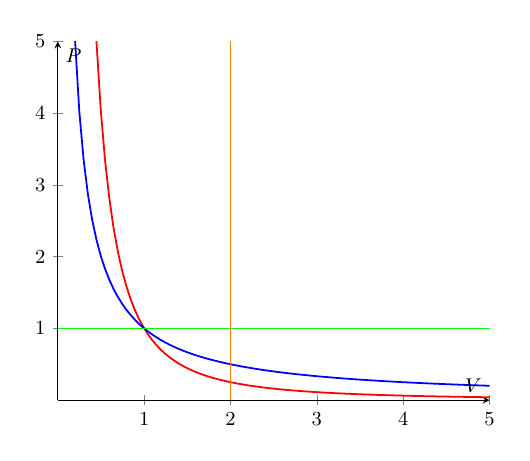
\begin{tikzpicture}[scale=0.8, font=\small]
                \begin{axis}[
                    axis lines = middle,
                    xlabel = {$V$},
                    ylabel = {$P$},
                    xtick={},
                    ytick={},
                    xmin=0, xmax=5,
                    ymin=0, ymax=5,
                ]
                    % Adiabatiche
                    \addplot[domain=0.1:5, thick,samples=100, red] {1/x^2};
                    % Isoterme
                    \addplot[domain=0.1:5, thick,samples=100, blue] {1/x};
                    % Isocore
                    \addplot[domain=0:5, thick,samples=100, green] {1};
                    % Isobare
                    \addplot[thick,samples=100, orange] coordinates {(2,0) (2,5)};
                \end{axis}
            \end{tikzpicture}
            \caption{Trasformazioni dei gas ideali}
        \end{figure}
        La curva rossa rappresenta la trasformazione adiabatiche, la curva blu rappresenta la trasformazione isoterma, la retta verde rappresenta la trasformazione isocora e la retta arancione rappresenta la trasformazione isobara.
    \subsection{Trasformazioni politropiche e generali}
        Le trasformazioni politropiche sono tali che per tutta la loro durata il calore specifico rimane costante ($c_k$) e quindi per la prima legge della termodinamica possiamo scrivere:
        \begin{align*}
            nc_vdT = nc_kdT - pdV
        \end{align*}
        definiamo ora la costante $k$ come la somma del rapporto tra la costante $R$ ed la differenza tra i calori specifici $c_v$ e $c_k$ con 1 ($k=\frac{R}{c_v-c_k}+1$) e quindi scriviamo:
        \begin{align*}
            PV^{k} = \text{costante}
        \end{align*}
        per le altre trasformazioni generali ricorriamo al primo principio della termodinamica (\ref{eq:prima_legge_termo}).